\documentclass[10pt]{article}
\usepackage{../pplmanual}
\NeedsTeXFormat{LaTeX2e}
\typeout{^^J^^J
Parallel Programming Laboratory^^J
Manual Style^^J
Written by Milind A. Bhandarkar, 12/00^^J}

%%% Make it possible for both ps and pdf to be generated
\newif\ifpdf
\ifx\pdfoutput\undefined
  \pdffalse
\else
  \pdfoutput=1
  \pdftrue
\fi

\ifpdf
  \pdfcompresslevel=9
\fi

%%% Imported from fullpage.sty, since it is not always available
\topmargin 0pt
\advance \topmargin by -\headheight
\advance \topmargin by -\headsep

\textheight 8.9in

\oddsidemargin 0pt
\evensidemargin \oddsidemargin
\marginparwidth 1.0in

\textwidth 6.5in
%%% end import from fullpage

%%% Commonly Needed packages
\usepackage{graphicx,color,calc}
\usepackage{makeidx}
\usepackage{alltt}

%%% Commands for uniform looks of C++, Charm++, and Projections
\newcommand{\CC}{C\kern -0.0em\raise 0.5ex\hbox{\normalsize++}}
\newcommand{\emCC}{C\kern -0.0em\raise 0.4ex\hbox{\normalsize\em++}}
\newcommand{\charmpp}{\sc Charm++}
\newcommand{\projections}{\sc Projections}
\newcommand{\converse}{\sc Converse}
\newcommand{\ampi}{\sc AMPI}

%%% Commands to produce margin symbols
\newcommand{\new}{\marginpar{\fbox{\bf$\mathcal{NEW}$}}}
\newcommand{\important}{\marginpar{\fbox{\bf\Huge !}}}
\newcommand{\experimental}{\marginpar{\fbox{\bf\Huge $\beta$}}}

%%% Commands for manual elements
\newcommand{\zap}[1]{ }
\newcommand{\function}[1]{{\noindent{\textsf{#1}}\\}}
\newcommand{\cmd}[1]{{\noindent{\textsf{#1}}\\}}
\newcommand{\args}[1]{\hspace*{2em}{\texttt{#1}}\\}
\newcommand{\param}[1]{{\texttt{#1}}}
\newcommand{\kw}[1]{{\textsf{#1}}}
\newcommand{\uw}[1]{{\textsl{#1}}}
\newcommand{\desc}[1]{\indent{#1}}

%%% Commands needed for Maketitle
\newcommand{\@version}{}
\newcommand{\@credits}{}
\newcommand{\version}[1]{\renewcommand{\@version}{#1}}
\newcommand{\credits}[1]{\renewcommand{\@credits}{#1}}

%%% Print the License Page
\newcommand{\@license}{%
 \begin{center}
   {University of Illinois}\\
   {\charmpp/\converse\ Parallel Programming System Software}\\
   {Non-Exclusive, Non-Commercial Use License}\\
 \end{center}
 \rule{\textwidth}{1pt}
{\tiny
Upon execution of this Agreement by the party identified below (``Licensee''),
The Board of Trustees of the University of Illinois  (``Illinois''), on behalf
of The Parallel Programming Laboratory (``PPL'') in the Department of Computer
Science, will provide the \charmpp/\converse\ Parallel Programming System
software (``\charmpp'') in Binary Code and/or Source Code form (``Software'')
to Licensee, subject to the following terms and conditions. For purposes of
this Agreement, Binary Code is the compiled code, which is ready to run on
Licensee's computer.  Source code consists of a set of files which contain the
actual program commands that are compiled to form the Binary Code.

\begin{enumerate}
  \item
    The Software is intellectual property owned by Illinois, and all right,
title and interest, including copyright, remain with Illinois.  Illinois
grants, and Licensee hereby accepts, a restricted, non-exclusive,
non-transferable license to use the Software for academic, research and
internal business purposes only, e.g. not for commercial use (see Clause 7
below), without a fee.

  \item 
    Licensee may, at its own expense, create and freely distribute
complimentary works that interoperate with the Software, directing others to
the PPL server (\texttt{http://charm.cs.uiuc.edu}) to license and obtain the
Software itself. Licensee may, at its own expense, modify the Software to make
derivative works.  Except as explicitly provided below, this License shall
apply to any derivative work as it does to the original Software distributed by
Illinois.  Any derivative work should be clearly marked and renamed to notify
users that it is a modified version and not the original Software distributed
by Illinois.  Licensee agrees to reproduce the copyright notice and other
proprietary markings on any derivative work and to include in the documentation
of such work the acknowledgement:

\begin{quote}
``This software includes code developed by the Parallel Programming Laboratory
in the Department of Computer Science at the University of Illinois at
Urbana-Champaign.''
\end{quote}

Licensee may redistribute without restriction works with up to 1/2 of their
non-comment source code derived from at most 1/10 of the non-comment source
code developed by Illinois and contained in the Software, provided that the
above directions for notice and acknowledgement are observed.  Any other
distribution of the Software or any derivative work requires a separate license
with Illinois.  Licensee may contact Illinois (\texttt{kale@cs.uiuc.edu}) to
negotiate an appropriate license for such distribution.

  \item
    Except as expressly set forth in this Agreement, THIS SOFTWARE IS PROVIDED
``AS IS'' AND ILLINOIS MAKES NO REPRESENTATIONS AND EXTENDS NO WARRANTIES OF
ANY KIND, EITHER EXPRESS OR IMPLIED, INCLUDING BUT NOT LIMITED TO WARRANTIES OR
MERCHANTABILITY OR FITNESS FOR A PARTICULAR PURPOSE, OR THAT THE USE OF THE
SOFTWARE WILL NOT INFRINGE ANY PATENT, TRADEMARK, OR OTHER RIGHTS.  LICENSEE
ASSUMES THE ENTIRE RISK AS TO THE RESULTS AND PERFORMANCE OF THE SOFTWARE
AND/OR ASSOCIATED MATERIALS.  LICENSEE AGREES THAT UNIVERSITY SHALL NOT BE HELD
LIABLE FOR ANY DIRECT, INDIRECT, CONSEQUENTIAL, OR INCIDENTAL DAMAGES WITH
RESPECT TO ANY CLAIM BY LICENSEE OR ANY THIRD PARTY ON ACCOUNT OF OR ARISING
FROM THIS AGREEMENT OR USE OF THE SOFTWARE AND/OR ASSOCIATED MATERIALS.

  \item 
    Licensee understands the Software is proprietary to Illinois. Licensee
agrees to take all reasonable steps to insure that the Software is  protected
and secured from unauthorized disclosure, use, or release and  will treat it
with at least the same level of care as Licensee would use to  protect and
secure its own proprietary computer programs and/or information, but using no
less than a reasonable standard of care.  Licensee agrees to provide the
Software only to any other person or entity who has registered with Illinois.
If licensee is not registering as an individual but as an institution or
corporation each member of the institution or corporation who has access to or
uses Software must agree to and abide by the terms of this license. If Licensee
becomes aware of any unauthorized licensing, copying or use of the Software,
Licensee shall promptly notify Illinois in writing. Licensee expressly agrees
to use the Software only in the manner and for the specific uses authorized in
this Agreement.

  \item
    By using or copying this Software, Licensee agrees to abide by the
copyright law and all other applicable laws of the U.S. including, but not
limited to, export control laws and the terms of this license. Illinois  shall
have the right to terminate this license immediately by written  notice upon
Licensee's breach of, or non-compliance with, any terms of the license.
Licensee may be held legally responsible for any  copyright infringement that
is caused or encouraged by its failure to  abide by the terms of this license.
Upon termination, Licensee agrees to  destroy all copies of the Software in its
possession and to verify such  destruction in writing.

  \item
  The user agrees that any reports or published results obtained with  the
Software will acknowledge its use by the appropriate citation as  follows:

\begin{quote}
``\charmpp/\converse\ was developed by the Parallel Programming Laboratory in
the Department of Computer Science at the University of  Illinois at
Urbana-Champaign.''
\end{quote}

Any published work which utilizes \charmpp\ shall include the following
reference:

\begin{quote}
``L. V. Kale and S. Krishnan. \charmpp: Parallel Programming with Message-Driven
Objects. In 'Parallel Programming using \CC' (Eds. Gregory V. Wilson and Paul
Lu), pp 175-213, MIT Press, 1996.''
\end{quote}

Any published work which utilizes \converse\ shall include the following
reference:

\begin{quote}
``L. V. Kale, Milind Bhandarkar, Narain Jagathesan, Sanjeev Krishnan and Joshua
Yelon. \converse: An Interoperable Framework for Parallel Programming.
Proceedings of the 10th International Parallel Processing Symposium, pp
212-217, April 1996.''
\end{quote}

Electronic documents will include a direct link to the official \charmpp\ page
at \texttt{http://charm.cs.uiuc.edu/}

  \item
    Commercial use of the Software, or derivative works based thereon,
REQUIRES A COMMERCIAL LICENSE.  Should Licensee wish to make commercial use of
the Software, Licensee will contact Illinois (kale@cs.uiuc.edu) to negotiate an
appropriate license for such use. Commercial use includes: 

    \begin{enumerate}
      \item
	integration of all or part of the Software into a product for sale,
lease or license by or on behalf of Licensee to third parties, or 

      \item
	distribution of the Software to third parties that need it to
commercialize product sold or licensed by or on behalf of Licensee.
    \end{enumerate}

  \item
    Government Rights. Because substantial governmental funds have been  used
in the development of \charmpp/\converse, any possession, use or sublicense of
the Software by or to the United States government shall be subject to such
required restrictions.

  \item
    \charmpp/\converse\ is being distributed as a research and teaching tool
and as such, PPL encourages contributions from users of the code that might, at
Illinois' sole discretion, be used or incorporated to make the basic  operating
framework of the Software a more stable, flexible, and/or useful  product.
Licensees who contribute their code to become an internal  portion of the
Software agree that such code may be distributed by  Illinois under the terms
of this License and may be required to sign an  ``Agreement Regarding
Contributory Code for \charmpp/\converse\ Software'' before Illinois  can
accept it (contact \texttt{kale@cs.uiuc.edu} for a copy).
\end{enumerate}

UNDERSTOOD AND AGREED.

Contact Information:

The best contact path for licensing issues is by e-mail to
\texttt{kale@cs.uiuc.edu} or send correspondence to:

\begin{quote}
Prof. L. V. Kale\\
Dept. of Computer Science\\
University of Illinois\\
1304 W. Springfield Ave\\
Urbana, Illinois 61801 USA\\
FAX: (217) 333-3501
\end{quote}
}%tiny
 \newpage
}% end of license

\renewcommand{\maketitle}{\begin{titlepage}%
 \begin{flushright}
   {\Large
     Parallel Programming Laboratory\\
     University of Illinois at Urbana-Champaign\\
   }
 \end{flushright}
 \rule{\textwidth}{3pt}
 \vspace{\fill}
 \begin{flushright}
   \textsf{\Huge \@title \\}
 \end{flushright}
 \vspace{\fill}
 \@credits \\
 \rule{\textwidth}{3pt}
 \begin{flushright}
   {\large Version \@version}
 \end{flushright}
 \end{titlepage}
 \@license

 \tableofcontents
 \newpage
}% maketitle



\title{BigSim Parallel Simulator for Extremely Large Parallel Machines}
\version{1.01}
% #CLM# \credits{Charm++ BigSim Emulator was developed by Arun Singla, Neelam Saboo
        \credits{The Charm++ BigSim Emulator was developed by Arun Singla, Neelam Saboo
and Joshua Unger under the guidance of Prof. L. V. Kale. The new Converse 
% #CLM# BigSim Emulator is completely rewritten by Gengbin Zheng. Converse BigSim 
        BigSim Emulator was completely rewritten by Gengbin Zheng. The Converse BigSim 
Emulator is the only version under maintenance now. Charm++ and Adaptive MPI
% #CLM# (AMPI) was ported onto the BigSim Emulator by Gengbin Zheng. The parallel
        (AMPI) were ported onto the BigSim Emulator by Gengbin Zheng. The parallel
performance simulator was developed by Gengbin Zheng and 
Gunavardhan Kakulapati. A postmortem network simulator was developed by 
Terry Wilmarth, Eric Bohm and Gengbin Zheng}

\begin{document}
\maketitle

\section{Introduction}

%One approach for building the next generation of parallel computers
%is based on large aggregates of multiprocessor chips with support
%for hardware multithreading. 
%An initial design for IBM's Blue Gene/C project exemplifies this approach.
%Blue Gene/C was a proposed one million processor machine from IBM.

Parallel machines with an extremely large number of processors are now
being designed and built. For example, the BlueGene/L (BG/L) machine
% #CLM# being built by IBM will have 64,000 dual-processor nodes with 360 teraflops
built by IBM has 64,000 dual-processor nodes with 360 teraflops of
peak performance. Another more radical design from IBM,
code-named Cyclops (BlueGene/C), had over one million floating point units,
fed by 8 million instructions streams supported by individual thread units,
targeting 1 petaflops of peak performance.


It is important that one can study the programming issues and performance
of parallel applications on such machines even before the machine is built.
Thus, we have developed a parallel simulator -- BigSim, to facilitate this research.

% #CLM# Since our research was initiated by Blue Gene/C project, in this manual, 
Since our research was initiated by the BlueGene/C project, in previous editions of this manual
we also called our simulator as Blue Gene Simulator.
Our simulator is capable of simulating a broad class of "Massively Parallel
Processors-In-Memory", or MPPIM machines. 

\subsection{Simulator system components}

Our simulator system includes these components: 
\begin{enumerate}
% #CLM# \item a parallel emulator which emulates the low level machine API; 
        \item a parallel emulator which emulates a low level machine API targeting an architecture like BlueGene; 
\item a message driven programming language (Charm++) running on top of the emulator; 
% #CLM# \item adaptive MPI (an implementation of MPI on top of Charm++) environment; 
        \item the Adaptive MPI (an implementation of MPI on top of Charm++) environment; 
% #CLM# Remove support for Online Simulator
% #CLM# \item a parallel online mode simulator for performance prediction; 
% #CLM# \item a parallel postmoterm mode network simulator for performance prediction. 
        \item a parallel postmoterm mode simulator for performance prediction, including network simulation. 
\end{enumerate}

\subsection{History}

% #CLM# The first version of Blue Gene emulator was written in Charm++, a 
        The first version of the BlueGene emulator was written in Charm++, a 
parallel object language, in fall 2001. 

% #CLM# The second version of Blue Gene emulator was completely rewritten on top 
        The second version of the BlueGene emulator was completely rewritten on top 
of Converse instead of Charm++ in spring 2002. 
% #CLM# While the API supported by the original emulator remains almost same,
        While the API supported by the original emulator remains almost the same,
many new features were added.
% - support of thread-committed messages that 
%can be send to a specific thread in a Blue Gene node; support of Blue Gene 
%node level broadcast.
The new emulator was implemented on a portable low layer communication 
library - Converse, in order to achieve better 
performance by avoiding the cross layer overhead.
%Another advantage is that the lighter weighted emulator makes it easier
%to port higher level of programming language onto the emulator.

% #CLM# Charm++ was soon ported to the emulator in 2002 which provided the
        Charm++ was ported to the emulator in 2002, providing the
 first parallel language model on top of the emulator.

A performance simulation capability was added to the emulator in spring 2003.
The new simulator was renamed to BigSim at the same time.
During the same year, we developed a POSE-based postmortem mode network
simulator called BigNetSim. In fall 2006, we renamed BigNetSim as simply
BigSim simulator.

In the following sections, we will first describe how to download and compile
% #CLM# Blue Gene simulator(Section ~\ref{install}). Section~\ref{bgemulator} will describe
    the BigSim system (Section~\ref{install}). Section~\ref{bgemulator} describes
% #CLM# the low level machine API in detail. 
    the BigSim Emulator and the low level machine API in detail. 


\section{BigSim Simulator Installation and Usage}
\label{install}

\subsection{Installing Charm++ and BigSim}

BigSim Simulator is distributed as a part of the Charm++ standard distribution.
One needs to download Charm++ and compile BigSim simulator.
One should begin with downloading Charm++ from the website:
http://charm.cs.uiuc.edu.

Please refer to ``Charm++ Installation and Usage Manual" and also the file
README in the source code for detailed instructions on how to compile Charm++.
In short, the ``build" script is the main tool for compiling \charmpp{}.  You
need to provide target and platform options: \begin{verbatim} ./build <target>
<platform> [options ...] [charmc-options ...] \end{verbatim}

For example, to compile on a Linux machine, type:
\begin{verbatim}
./build charm++ net-linux -O
\end{verbatim}

which builds essential \charmpp{} kernel using UDP sockets as 
communication method, 
alternatively, you can build Charm++ kernel on MPI using:
\begin{verbatim}
./build charm++ mpi-linux -O
\end{verbatim}

For other platforms, change net-linux to whatever platform you are compiling 
on. See the charm/README file for a complete list of supported platforms.

\subsubsection{Build Only the BigSim Emulator}

BigSim emulator is implemented on top of Converse in Charm++.
To compile BigSim emulator, one can compile emulator libraries
directly on top of normal Charm++ using ``bigsim'' as the compilation
target, like
\begin{verbatim}
./build bigsim net-linux -O
\end{verbatim}

With emulator libraries, one can write BigSim applications using its
low level emulator message passing API.

\subsubsection{Build Charm++ on BigSim Emulator}

In order to build Charm++ on top of BigSim Emulator (which itself is 
implemented on top of Converse), a special build option ``bigsim''
needs to be specified:
\begin{verbatim}
./build bigsim net-linux bigsim -O
\end{verbatim}

The first ``bigsim" is the compilation target that tells ``build" to
compile BigSim emulator libraries in addition to \charmpp{} kernel libraries;
The second ``bigsim" is a build option to platform ``net-linux", which tells
``build" to build the Charm++ on top of BigSim Emulator. 
To build AMPI on BigSim, use ``bgampi" as make target, which subsumes target
of ``bigsim":
\begin{verbatim}
./build bgampi net-linux bigsim -O
\end{verbatim}

For the above ``build" command, it creates a directory named 
``net-linux-bigsim" under charm, which contains all the header files and
libraries needed for compiling a user application.

\subsection{Compiling BigSim Applications}

\charmpp{} provides a compiler script {\tt charmc} to compile all programs.

There are three methods to write a BigSim application:

\subsubsection{Writing a BigSim application using low level machine API}
The low level machine API mimics the actual machine low level programming
API. It is defined in section~\ref{bgemulator}. Writing a program in the 
low level machine API, you just need to link \charmpp{}'s BigSim emulator
libraries, which provide the emulation of the machine API using Converse as
the communication layer.

In order to link against the BigSim library, specify 
\texttt{-language bigsim} as an argument to the {\tt charmc} linker, 
for example:
\begin{verbatim}
charmc -o hello hello.C -language bigsim
\end{verbatim}

Sample applications in low level machine API can be found under directory
charm/pgms/converse/bluegene.

\subsubsection{Writing a BigSim application in Charm++}

One can write a normal \charmpp{} application which can automatically 
run on the emulator after compilation. \charmpp{} implements
an object-based message-driven execution model. In \charmpp{} applications,
there are collections of C++ objects, which communicate by remotely invoking
methods on other objects by messages.

In order to compile a program written in \charmpp{} on Blue Gene simulator, 
specify \texttt{-language charm++} as an argument to the {\tt charmc} linker:
\begin{verbatim}
charmc -o hello hello.C -language charm++
\end{verbatim}
This will link both \charmpp{} runtime libraries and BigSim simulator 
libraries.

Sample applications in \charmpp{} can be found under directory
charm/pgms/charm++, specifically charm/pgms/charm++/littleMD.

\subsubsection{Writing a Blue Gene application in MPI}

One can also write a MPI application for Blue Gene Simulator.
The Adaptive MPI, or AMPI is implemented on top of Charm++ that supports
dynamic load balancing and multithreading for MPI applications. This is based
on the user-level migrating threads and load balancing capabilities provided
by the \charmpp{} framework. This allows legacy MPI programs to run 
on top of Blue Gene \charmpp{} and take advantage of the \charmpp{}'s
virtualization and adaptive load balancing capability.

Current AMPI implements most features in the MPI version 1.0, with a few
extensions for migrating threads and asynchronous reduction.

In order to compile an AMPI application on Blue Gene simulator, you need 
to link against the AMPI library as well as Blue Gene \charmpp{} runtime
libraries by specifying \texttt{-language ampi} as an argument to 
the {\tt charmc} linker:
\begin{verbatim}
charmc -o hello hello.C -language ampi
\end{verbatim}

Sample applications in AMPI can be found under directory
charm/pgms/charm++/ampi, specifically charm/pgms/charm++/Cjacobi3D.

\subsection{Run a BigSim Application}

To run a parallel Blue Gene application, \charmpp{} provides a utility program
called {\tt charmrun} to start the parallel program. 
For detailed description on how to run a \charmpp{} application, 
refer to the file charm/README in the source code distribution.

To run a Blue Gene application, you need to specify these parameters to 
{\tt charmrun} to define the simulated Blue Gene machine size:
\begin{enumerate}
\item {\tt +x, +y} and {\tt +z}:  define the size of the machine in three dimensions, these define the number of nodes along each dimension of the machine;
\item {\tt +wth} and {\tt +cth}:  For one node, these two parameters define the number of worker processors({\tt +wth}) and the number of communication processors({\tt +cth}).
\item {\tt +bgcorrect}: starts the simulation mode for performance prediction. Otherwise the program runs without doing parallel event simulation for performance prediction of the application.
\item {\tt +bgwalltime}: used only in simulation mode, when specified, use wallclock measurement of the time taken on the simulating machine to estimate the time it takes to run on the target machine.
\item {\tt +bgcounter}:  used only in simulation mode, when specified, use the performance counter to estimate the time on target machine. This is currently only supported when perfex is installed, like Origin2000.
\end{enumerate}

For example, to simulate a Blue Gene/L machine of size 64K in 40x40x40, with 
one worker processor and one I/O processor on each node, and use 100 
real processors to simulate:
\begin{verbatim}
./charmrun +p100 ./hello +x40 +y40 +z40 +cth1 +wth1
\end{verbatim}

To run an AMPI program, you may also want to specify the number of virtual 
processors to run the MPI by using {\tt +vp}, for example:
\begin{verbatim}
./charmrun +p100 ./hello +x40 +y40 +z40 +cth1 +wth1 +vp 128000
\end{verbatim}
starts the simulation of Blue Gene/L of size 40x40x40 with 2 processors 
in each node, running 128000 MPI threads (2 MPI threads on each Blue Gene node),
 using 100 real processors to simulate. In this case, {\tt MPI\_Comm\_size()}
returns 128000 for {\tt MPI\_COMM\_WORLD}. If you donot specify the {\tt +vp}
option, the number of virtual processors will be equal to the number of 
processors of the simulated machine, in this case 64000.




\section{Blue Gene Emulator}
\label{bgemulator}

The Blue Gene emulator environment is designed with the following
objectives:

\begin{enumerate}
\item To support a realistic Blue Gene API on existing parallel machines

\item To obtain first-order performance estimates of algorithms

\item To facilitate implementations of alternate programming models for
      Blue Gene
\end{enumerate}

The ``Blue Gene'' machine supported by the emulator consists of
three-dimensional grid of 1-chip nodes.  The user may specify the size
of the machine along each dimension (e.g. 34x34x36).  The chip supports
$k$ threads (e.g. 200), each with its own integer unit.  The proximity of
the integer unit with individual memory modules within a chip is not
currently modeled.

The API supported by the emulator can be broken down into several
components:

\begin{enumerate}
\item Low-level API for chip-to-chip communication
\item Mid-level API that supports local micro-tasking with a chip level
scheduler with features such as: read-only variables, reductions, broadcasts,
distributed tables, get/put operations
\item Migratable objects with automatic load balancing support
\end{enumerate}

Of these, the first two have been implemented.  The simple time stamping
algorithm, without error correction, has been implemented.  More
sophisticated timing algorithms, specifically aimed at error correction,
and more sophisticated features (2, 3, and others), as well as libraries
of commonly needed parallel operations are part of the proposed work for
future.

The following sections define the appropriate parts of the API, with
example programs and instructions for executing them.

\subsection{Blue Gene Programming Environment}

The basic philosophy of the Blue Gene Emulator is to hide intricate details
of the Blue Gene machine from the
application developer. Thus, the application developer needs to provide
intialization details and handler
functions only and gets the result as though running on a real machine.
Communication, Thread creation,
Time Stamping, etc are done by the emulator.

\subsubsection{Blue Gene API: Level 0}

\function{void addBgNodeInbuffer(bgMsg *msgPtr, int nodeID)}
\desc{
        low-level primitive invoked by Blue Gene emulator to put the 
        message to the inbuffer queue of a node.

        msgPtr - pointer to the message to be sent to target node; 

        nodeID - node ID of the target node, it is the serial number of a 
                 bluegene node in the emulator's physical node.
}

\function{void addBgThreadMessage(bgMsg *msgPtr, int threadID)}
\desc{
        add a message to a thread's affinity queue, these messages can be 
 	only executed by a specific thread indicated by threadID.
}

\function{void addBgNodeMessage(bgMsg *msgPtr)}
\desc{
	add a message to a node's non-affinity queue, these messages can be 
	executed by any thread in the node.
}

\function{boolean checkReady()}
\desc{
        invoked by communication thread to see if there is any unattended
        message in inBuffer.
}

\function{bgMsg * getFullBuffer()}
\desc{
	invoked by communication thread to retrieve the unattended message 
	in inBuffer.
}

\function{CmiHandler msgHandlerFunc(char *msg)}
\desc{
	Handler function type that user can register to handle the message.
}

\function{void sendPacket(int x, int y, int z, int msgSize,bgMsg *msg)}
\desc{
	chip-to-chip communication function. It send a message to Node[x][y][z].
        
	bgMsg is the message type with message envelop used internally.
}

\subsubsection{Initialization API: Level 1a}

All the functions defined in API Level 0 are used internally for the 
implementation of bluegene node communication and worker threads.

From this level, the functions defined are exposed to users to write bluegene
programs on the emulator.

Considering that the emulator machine will emulate several Bluegene nodes on
each physical node, the emulator program defines this function 
\function{BgEmulatorInit(int argc, char **argv)} to initialize each emulator
node. In this function, user program can define the Bluegene machine size,
number of communication/worker threads, and check the command line arguments.

The size of the Blue Gene machine being emulated and the number of thread per
node is determined either by the command line arguments or calling following
functions:

\function{void BgSetSize(int sx, int sy, int sz)}
\desc{
	set Blue Gene Machine size;
}

\function{void BgSetNumWorkThread(int num)}
\desc{
	set number of worker threads per node;
}

\function{void BgSetNumCommThread(int num)}
\desc{
	set number of communication threads per node;
}

\function{int BgRegisterHandler(BgHandler h)}
\desc{
	register user message handler functions; 
}

For each Blue Gene node, the execution starts at 
\function{BgNodeStart(int argc, char **argv)} called by the emulator,
where application handlers can be registered and computation 
is triggered by creating a task at required nodes.

Similar to pthread's thread specifc data, each bluegene node has its
own node specific data associated with it. To do this, the user needs to define its 
own node-specific variables encapsulated in a struct definition and register
 the pointer to the data with the emulator by following function:

\function{void BgSetNodeData(char *data)}

To retrieve the node specific data, call:

\function{char *BgGetNodeData();}

After completion of execution, user program invokes a function:

\function{void BgShutdown()}

to terminate the emulator.

\subsubsection{Handler Function API: Level 1a}

The following functions can be called in user's application program to retrieve
the Blue Gene machine information, get thread execution time, and perform
the communication.

\function{void BgGetSize(int *sx, int *sy, int *sz);}

\function{int BgGetNumWorkThread();}

\function{int BgGetNumCommThread();}

\function{int BgGetThreadID();}

\function{double BgGetTime();}

\function{void BgSendPacket(int x, int y, int z, int threadID, int handlerID, WorkType type, int numbytes, char* data);}
\desc{
This sends a trunk of data to Node[x, y, z] and also specifies the
handler function to be used for this message i.e. the handlerID;
threadID specifes the desired thread to handle the message, ANYTHREAD means
no preference.

To specify the thread category:
\begin{description}
\item[1:] a small piece of work that can be done by
communication thread itself, so NO scheduling overhead.
\item[0:] a large piece of work, so communication thread
schedules it for a worker thread
\end{description}
}


\subsection{Writing a Blue Gene Application}

\subsubsection{Application Skeleton}

\begin{alltt}
Handler function prototypes;
Node specific data type declarations;

void  BgEmulatorInit(int argc, char **argv)  function
  Configure bluegene machine parameters including size, number of threads, etc.
  You also neet to register handlers here.

void *BgNodeStart(int argc, char **argv) function
  The usual practice in this function is to send an intial message to trigger 
  the execution.
  You can also register node specific data in this function.

Handler Function 1, void handlerName(char *info)
Hanlder Function 2, void handlerName(char *info)
..
Handler Function N, void handlerName(char *info)

\end{alltt}

\subsubsection{Sample Application 1}

\begin{verbatim}
/* Application: 
 *   Each node starting at [0,0,0] sends a packet to next node in
 *   the ring order.
 *   After node [0,0,0] gets message from last node
 *   in the ring, the application ends.
 */


#include "blue.h"

#define MAXITER 2

int iter = 0;
int passRingHandler;

void passRing(char *msg);

void nextxyz(int x, int y, int z, int *nx, int *ny, int *nz)
{
  int numX, numY, numZ;

  BgGetSize(&numX, &numY, &numZ);
  *nz = z+1; *ny = y; *nx = x;
  if (*nz == numZ) {
    *nz = 0; (*ny) ++;
    if (*ny == numY) {
      *ny = 0; (*nx) ++;
      if (*nx == numX) *nx = 0;
    }
  }
}

void BgEmulatorInit(int argc, char **argv)
{
  passRingHandler = BgRegisterHandler(passRing);
}

/* user defined functions for bgnode start entry */
void BgNodeStart(int argc, char **argv)
{
  int x,y,z;
  int nx, ny, nz;
  int data, id;

  BgGetXYZ(&x, &y, &z);
  nextxyz(x, y, z, &nx, &ny, &nz);
  id = BgGetThreadID();
  data = 888;
  if (x == 0 && y==0 && z==0) {
    BgSendPacket(nx, ny, nz, -1,passRingHandler, LARGE_WORK, 
				sizeof(int), (char *)&data);
  }
}

/* user write code */
void passRing(char *msg)
{
  int x, y, z;
  int nx, ny, nz;
  int id;
  int data = *(int *)msg;

  BgGetXYZ(&x, &y, &z);
  nextxyz(x, y, z, &nx, &ny, &nz);
  if (x==0 && y==0 && z==0) {
    if (++iter == MAXITER) BgShutdown();
  }
  id = BgGetThreadID();
  BgSendPacket(nx, ny, nz, -1, passRingHandler, LARGE_WORK, 
				sizeof(int), (char *)&data);
}

\end{verbatim}


\subsubsection{Sample Application 2}

\begin{verbatim}

/* Application: 
 *   Find the maximum element.
 *   Each node computes maximum of it's elements and
 *   the max values it received from other nodes
 *   and sends the result to next node in the reduction sequence.
 * Reduction Sequence: Reduce max data to X-Y Plane
 *   Reduce max data to Y Axis
 *   Reduce max data to origin.
 */


#include <stdlib.h>
#include "blue.h"

#define A_SIZE 4

#define X_DIM 3
#define Y_DIM 3
#define Z_DIM 3

int REDUCE_HANDLER_ID;
int COMPUTATION_ID;

extern "C" void reduceHandler(char *);
extern "C" void computeMax(char *);

class ReductionMsg {
public:
  int max;
};

class ComputeMsg {
public:
  int dummy;
};

void BgEmulatorInit(int argc, char **argv)
{
  if (argc < 2) { 
    CmiAbort("Usage: <program> <numCommTh> <numWorkTh>\n"); 
  }

  /* set machine configuration */
  BgSetSize(X_DIM, Y_DIM, Z_DIM);
  BgSetNumCommThread(atoi(argv[1]));
  BgSetNumWorkThread(atoi(argv[2]));

  REDUCE_HANDLER_ID = BgRegisterHandler(reduceHandler);
  COMPUTATION_ID = BgRegisterHandler(computeMax);

}

void BgNodeStart(int argc, char **argv) {
  int x, y, z;
  BgGetXYZ(&x, &y, &z);

  ComputeMsg *msg = new ComputeMsg;
  BgSendLocalPacket(ANYTHREAD, COMPUTATION_ID, LARGE_WORK, 
			sizeof(ComputeMsg), (char *)msg);
}

void reduceHandler(char *info) {
  // assumption: THey are initialized to zero?
  static int max[X_DIM][Y_DIM][Z_DIM];
  static int num_msg[X_DIM][Y_DIM][Z_DIM];

  int i,j,k;
  int external_max;

  BgGetXYZ(&i,&j,&k);
  external_max = ((ReductionMsg *)info)->max;
  num_msg[i][j][k]++;

  if ((i == 0) && (j == 0) && (k == 0)) {
    // master node expects 4 messages:
    // 1 from itself;
    // 1 from the i dimension;
    // 1 from the j dimension; and
    // 1 from the k dimension
    if (num_msg[i][j][k] < 4) {
      // not ready yet, so just find the max
      if (max[i][j][k] < external_max) {
	max[i][j][k] = external_max;
      }
    } else {
      // done. Can report max data after making last comparison
      if (max[i][j][k] < external_max) {
	max[i][j][k] = external_max;
      }
      CmiPrintf("The maximal value is %d \n", max[i][j][k]);
      BgShutdown();
      return;
    }
  } else if ((i == 0) && (j == 0) && (k != Z_DIM - 1)) {
    // nodes along the k-axis other than the last one expects 4 messages:
    // 1 from itself;
    // 1 from the i dimension;
    // 1 from the j dimension; and
    // 1 from the k dimension
    if (num_msg[i][j][k] < 4) {
      // not ready yet, so just find the max
      if (max[i][j][k] < external_max) {
	max[i][j][k] = external_max;
      }
    } else {
      // done. Forwards max data to node i,j,k-1 after making last comparison
      if (max[i][j][k] < external_max) {
	max[i][j][k] = external_max;
      }
      ReductionMsg *msg = new ReductionMsg;
      msg->max = max[i][j][k];
      BgSendPacket(i,j,k-1,ANYTHREAD,REDUCE_HANDLER_ID,LARGE_WORK, 
				sizeof(ReductionMsg), (char *)msg);
    }
  } else if ((i == 0) && (j == 0) && (k == Z_DIM - 1)) {
    // the last node along the k-axis expects 3 messages:
    // 1 from itself;
    // 1 from the i dimension; and
    // 1 from the j dimension
    if (num_msg[i][j][k] < 3) {
      // not ready yet, so just find the max
      if (max[i][j][k] < external_max) {
	max[i][j][k] = external_max;
      }
    } else {
      // done. Forwards max data to node i,j,k-1 after making last comparison
      if (max[i][j][k] < external_max) {
	max[i][j][k] = external_max;
      }
      ReductionMsg *msg = new ReductionMsg;
      msg->max = max[i][j][k];
      BgSendPacket(i,j,k-1,ANYTHREAD,REDUCE_HANDLER_ID,LARGE_WORK, 
				sizeof(ReductionMsg), (char *)msg);
    }
  } else if ((i == 0) && (j != Y_DIM - 1)) {
    // for nodes along the j-k plane except for the last and first row of j,
    // we expect 3 messages:
    // 1 from itself;
    // 1 from the i dimension; and
    // 1 from the j dimension
    if (num_msg[i][j][k] < 3) {
      // not ready yet, so just find the max
      if (max[i][j][k] < external_max) {
	max[i][j][k] = external_max;
      }
    } else {
      // done. Forwards max data to node i,j-1,k after making last comparison
      if (max[i][j][k] < external_max) {
	max[i][j][k] = external_max;
      }
      ReductionMsg *msg = new ReductionMsg;
      msg->max = max[i][j][k];
      BgSendPacket(i,j-1,k,ANYTHREAD,REDUCE_HANDLER_ID,LARGE_WORK, 
				sizeof(ReductionMsg), (char *)msg);
    }
  } else if ((i == 0) && (j == Y_DIM - 1)) {
    // for nodes along the last row of j on the j-k plane,
    // we expect 2 messages:
    // 1 from itself;
    // 1 from the i dimension;
    if (num_msg[i][j][k] < 2) {
      // not ready yet, so just find the max
      if (max[i][j][k] < external_max) {
	max[i][j][k] = external_max;
      }
    } else {
      // done. Forwards max data to node i,j-1,k after making last comparison
      if (max[i][j][k] < external_max) {
	max[i][j][k] = external_max;
      }
      ReductionMsg *msg = new ReductionMsg;
      msg->max = max[i][j][k];
      BgSendPacket(i,j-1,k,ANYTHREAD,REDUCE_HANDLER_ID,LARGE_WORK, 
				sizeof(ReductionMsg), (char *)msg);
    }
  } else if (i != X_DIM - 1) {
    // for nodes anywhere the last row of i,
    // we expect 2 messages:
    // 1 from itself;
    // 1 from the i dimension;
    if (num_msg[i][j][k] < 2) {
      // not ready yet, so just find the max
      if (max[i][j][k] < external_max) {
	max[i][j][k] = external_max;
      }
    } else {
      // done. Forwards max data to node i-1,j,k after making last comparison
      if (max[i][j][k] < external_max) {
	max[i][j][k] = external_max;
      }
      ReductionMsg *msg = new ReductionMsg;
      msg->max = max[i][j][k];
      BgSendPacket(i-1,j,k,ANYTHREAD,REDUCE_HANDLER_ID,LARGE_WORK, 
				sizeof(ReductionMsg), (char *)msg);
    }
  } else if (i == X_DIM - 1) {
    // last row of i, we expect 1 message:
    // 1 from itself;
    if (num_msg[i][j][k] < 1) {
      // not ready yet, so just find the max
      if (max[i][j][k] < external_max) {
	max[i][j][k] = external_max;
      }
    } else {
      // done. Forwards max data to node i-1,j,k after making last comparison
      if (max[i][j][k] < external_max) {
	max[i][j][k] = external_max;
      }
      ReductionMsg *msg = new ReductionMsg;
      msg->max = max[i][j][k];
      BgSendPacket(i-1,j,k,-1,REDUCE_HANDLER_ID,LARGE_WORK, 
				sizeof(ReductionMsg), (char *)msg);
    }
  }
}

void computeMax(char *info) {
  int A[A_SIZE][A_SIZE];
  int i, j;
  int max = 0;

  int x,y,z; // test variables
  BgGetXYZ(&x,&y,&z);

  // Initialize
  for (i=0;i<A_SIZE;i++) {
    for (j=0;j<A_SIZE;j++) {
      A[i][j] = i*j;
    }
  }

//  CmiPrintf("Finished Initializing %d %d %d!\n",  x , y , z);

  // Find Max
  for (i=0;i<A_SIZE;i++) {
    for (j=0;j<A_SIZE;j++) {
      if (max < A[i][j]) {
	max = A[i][j];
      }
    }
  }

  // prepare to reduce
  ReductionMsg *msg = new ReductionMsg;
  msg->max = max;
  BgSendLocalPacket(ANYTHREAD, REDUCE_HANDLER_ID, LARGE_WORK, 
				sizeof(ReductionMsg), (char *)msg);

//  CmiPrintf("Sent reduce message to myself with max value %d\n", max);
}


\end{verbatim}


% #CLM# REMOVE ONLINE SIMULATOR; MOVE BGAPI HERE
% #CLM# Running with the simulator:


\converse{} provides a simple parallel machine simulator for developing
and debugging purposes. It simulates a message passing system. The simulated
machine is a collection of processing nodes connected with a communication
network. Each node is composed of an application processor, local memory, and 
a communication coprocessor. 
The simulator is a beta version, particularly using the simulator timers
for performance measurements has not been tested yet.

In order to run \converse{} programs with the simulator:
\begin{item}
\item link user program with <machine>/lib/libck-unimain.o
\item prepare a configuration file as described below
\item to run, type pgm +pN (and possibly other runtime options) where
   N is the number of processors.
\end{itemize}



The basic task of the simulator is to manage the message passing
obeying various machine and network parameters.
A message experiences delays in various components of the machine. These
include: 1) sender application processor, 2) sender communication coprocesssor, 
3) network, 4) receiver communication processor, and 5) receiver
application processor.
Each component of the delayed is modelled by the widely used formula
$\alpha + n\beta$ where $\alpha$ is the startup cost, and $\beta$ is the
cost per byte. 
In addition to message delay parameters, there are others related to the 
network capacity and random variations in network delays. These parameters
are specified in a configuration file named "sim.param" in the directory
of the user program. If the simulator can't find this file, it assumes
default values (mostly zero latencies).
Figure~\ref{fig:simconfig} lists a sample configuration. The lines
starting with the \# sign are treated as comments. Each line contains
a keyword followed by some numbers. The explanation of each keyword
is given below:

\begin{description}
\item[\verb+cpu_recv_cost+] $\alpha$ and  $\beta$ values  for the software
                            cost of a message-receive at the application
                            processor.
\item[\verb+cpu_send_cost+] $\alpha$ and  $\beta$ values  for the software
                            cost of a message-send at the application
                            processor.
\item[\verb+rcp_cost+] $\alpha$ and  $\beta$ values for a message-receive 
                       at the communication processor.
\item[\verb+scp_cost+] $\alpha$ and  $\beta$ values for a message-send
                       at the communication processor.
\item[\verb+net_cost+] $\alpha$ and  $\beta$ values for a message-send
                       in the netowrk.
\item[\verb+cpu_queue_threshold_number+] max number of messages queued
                       at the application processors's incoming message queue.
\item[\verb+cpu_queue_threshold_size+] max cumulative size of messages in bytes
                       queued at the application processors's incoming message 
                       queue.


\item[\verb+cpu_queue_threshold_number+] max number of messages in the incoming
                       message queue of communication processor.   


\item[\verb+rcp_queue_threshold_number+] max number of messages in the 
                       incoming-message-queue of communication processors.                    
\item[\verb+rcp_queue_threshold_size+] max cumulative size of messages in bytes
                       in the incoming-message-queue of communication 
                       processors.

\item[\verb+net_queue_threshold_number+] max number of transient messages in 
                       the network.

\item[\verb+net_queue_threshold_size+] max cumulative size of transient 
                       messages in bytes in the network.

\item[\verb+latency-fixed] no random variations in the network latency 
                           ($\alpha$)

\item[\verb+latency-rand+] network latency ($\alpha$) is incremented by
                       a random value distributed exponentially. The first
                       number after the keyword is the mean of the
                       exponential distribution. The second number is the
                       initial seed vbalue for the random number generator.


\item[\verb+processor_scale+] The simulator scales the measured time
                      execution of code-blocks by this value.

\item[\verb+periodic_interval+] \converse{} has periodic checks for
                      various purposes. This is the time on seconds
                      those checks are called.
\end{description}


\begin{figure}
\begin{alltt}
#latency parameters
cpu_recv_cost 1E-6 1E-7              
cpu_send_cost 1E-6 1E-7
rcp_cost      1E-3 1E-7
scp_cost      1E-6 1E-7
net_cost      1E-6 1E-7


#capacity parameters
# choose one 
cpu_nolimit
#cpu_queue_threshold_number 100000
#cpu_queue_threshold_size   100000


#choose one
scp_nolimit
#scp_queue_threshold_number 100000
#scp_queue_threshold_size   100000

#choose one
rcp_net_nolimit
#rcp_queue_threshold_number 100000
#rcp_queue_threshold_size   100000
#net_queue_threshold_number 100000
#net_queue_threshold_size   100000

#random variations in latency
#choose one
latency-fixed
#latency-rand   0.0001 123456

processor_scale 1.0
periodic_interval 0.1
\end{alltt}
\caption{A sample configuration file for the simulator}
\label{fig:simconfig}
\end{figure}


\section{BigSim Log Generation API}
\label{bgapi}


To be added ...


\section{BigSim Network Simulator}
\label{bignetsim}

The BigSim Network Simulator is also known as DetailedSim and lives 
in the pgms module in cvs at pose/DetailedSim. 
The Network simulator is actually more of an Inter-connection network 
simulator and hence more important in the context of large parallel
machines with interconnects. 
The BigSim simulator  along with the network simulator is together 
also known as BigNetSim.

Both the simulators run on top of the POSE framework, which is a Parallel
Discrete Event Simulation framework built on top of \charmpp{}.


\subsection{What does this software do?}
BigNetSim is an effort to simulate large current and future computer 
systems to study the behavior of applications developed for those systems. 
BigNetSim could be used to study
\begin{itemize}
\item  new types of interconnection topologies and routing algorithms 
along with different types of switching architecture.
\item application performance on different machines. This uses the API
provided in Section \ref{bgapi} to run the application on some number
of processors on some machine and generate (dump) all events (entry
method executions or message send/recv).  BigNetSim is used to 
model the machine that needs to be studied for this application and
these logs are then fed into this simulation, and it predicts the
performance of this application.
\end{itemize}

So, the two important uses are studying {\it interconnection networks} and
{\it perfomrance prediction for applications}.


\subsection{BigNetSim Design and Internals}
\begin{figure}[!t]
\centering  
  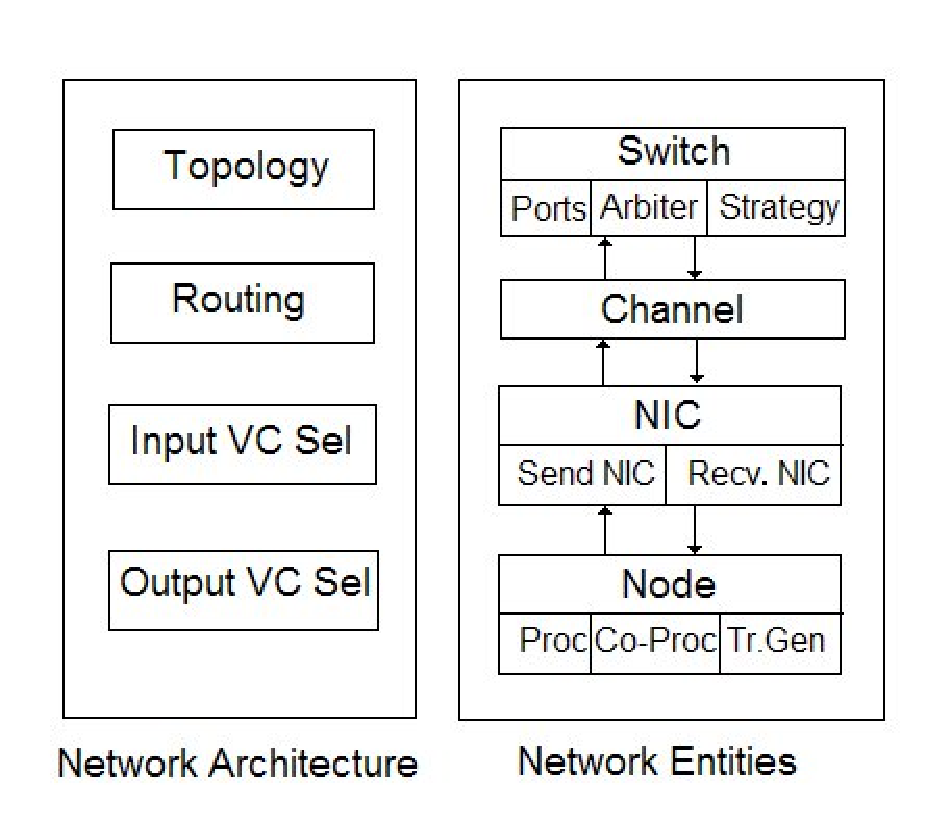
\includegraphics[width=3.2in]{figures/detailedsim_newer}
{\sffamily\bfseries\small \caption{BigNetSim conceptual model\label{fig:detailedsim_model}}}
\end{figure}

This section focuses on the interconnection network simulation.
The entities that form an interconnection network are:
\begin{itemize}
\item {\it switch:} A switch decides the routing on a packet. Switches could be
input buffered or output buffered. The former are implemented as individual posers
per port of each switch while the latter are implemented as a poser per switch.
In an {\it Input Buffered (IB)} switch, a packet in a switch is stored at the input 
port until its next route is decided and leaves the switch if it finds 
available space on the next switch in the route.
While in an {\it Output Buffered (OB)} switch, a packet in a switch decides beforehand 
on the next route to take and is buffered at the output port until space is
available on the next switch along the route.
Switches are modeled in much detail. Ports, buffers and
virtual channels at ports to avoid head-of-the-line blocking are
modeled.  Hardware collectives are implemented on the switch to
enable broadcasts, multicasts and other collective operations
efficiently. These are configurable and can be used if the system
being simulated supports them. We also support configurable
strategies for arbitration, input virtual channel selection and output
virtual channel selection. The configurability of the switch
provides a flexible design, satisfying the requirements of
a large number of networks.

\item {\it network card:} Network cards packetize and unpacketize messages.
A NIC is implemented as two posers. The sending and receiving entities in a
NIC are implemented as separate posers. A NIC is attached to each node.
\item {\it channel:} These are modelled as posers and connect a NIC to a switch
or a switch to another switch.
\item {\it compute node:} Each compute node connects to a network interface card.
A compute node simulates execution of entry methods on it. It is also attached
to a message traffic generator, which is used when only an interconnection
network is being simulated. This traffic generator can generate any message
pattern on each of the compute nodes.
The traffic generator can send
point-to-point messages, reductions, multicasts, broadcasts and other
collective traffic.  It supports k-shift, ring, bit-transpose,
bit-reversal, bit-complement and uniform random traffic.
These are based on common communication patterns found in
real applications. The frequency of message generation is determined
by a uniform or Poisson distribution.
\end{itemize}


\subsection{Topology, Routing and Virtual Channel Selection}
Topology, Routing strategies and input and output virtual channel seclection
strategies need to be decided for any inter-connection network. Once we
have all of these in place we can simulate an inter-connection network.

\subsubsection{Topology}
For every architecture one wants to design, a topology file has to written
which defines a few basic functions for that particular topology.
These are:

\function{void getNeighbours(int nodeid, int numP);}
\index{getNeighbours}
\desc{This is called initially for every switch and this populates the
data structure {\it next} in a switch which contains the connectivity
of that switch. The switch specified by {\it switch} has {\it numP} ports.}

\function{int getNext(int portid, int nodeid, int numP)}
\index{getNext}
\desc{Returns the index of the switch/node that is connected to the
switch {\it nodeid}, at {\it portid}. The number of ports this node has is {\it numP}.}

\function{int getNextChannel(int portid, int nodeid, int numP)}
\index{getNextChannel}
\desc{Returns the index of the channel that is connected to the
switch {\it nodeid}, at {\it portid}. The number of ports this node has is {\it numP}.}

\function{int getStartPort(int nodeid, int numP, int dest)}
\index{getStartPort}
\desc{Return the index of the port that is connected to this compute node from a switch}

\function{int getStartVc()}
\index{getStartVc}
\desc{Retuns the index of the first virtual channel (mostly 0).}

\function{int getStartSwitch(int nodeid)}
\index{getStartSwitch}
\desc{Retuns the index of the node/switch that is connected to the first port}

\function{int getStartNode()}
\index{getStartNode}
\desc{Returns the index of the first node. Each poser has a separate index, 
irrespective of the type of the poser.}

\function{int getEndNode()}
\index{getEndNode}
\desc{Retuns the index of the last node.}


\subsubsection{Routing}
Routing strategy needs to be specified for every interconnection network.
There is usually at least one routing strategy that needs to be defined
for every topology, Usually we have many more. The following functions need
to be defined for every routing strategy.

\function{int selectRoute(int current, int dest, int numP, Topology* top, Packet *p, map<int,int> \&bufsize, unsigned short *xsubi)}
\index{selectRoute}
\desc{Returns the portid that should be taken on switch {\it current} if the destination
is {\it dest}. The number of ports on a switch is {\it numP}. We also pass the pointer 
to the topology and to the Packet.}

\function{int selectRoute(int current, int dest, int numP, Topology* top, Packet *p, map<int,int> \&bufsize, map<int,int> \&portContention, unsigned short *xsubi)}
\index{selectRouteCont}
\desc{Returns the portid that should be taken on switch {\it current} if the destination
is {\it dest}. The number of ports on a switch is {\it numP}. We also pass the pointer 
to the topology and to the Packet. {\it Bufsize} is the state of the ports in
a switch, i.e. how many buffers on each port are full, while {\it portContention}
is used to give priority to certain ports, when more options are available.}

\function{int expectedTime(int src, int dest, POSE\_TimeType ovt, POSE\_TimeType origOvt, int length, int *numHops)}
\index{expectedTime}
\desc{Returns the expected time for a packet to travel from {\it src} to {\it dest},
when the number of hops it will need to travel is {\it numHops}.}

\function{int convertOutputToInputPort(int id, Packet *p, int numP, int *next)}
\index{convertOutputToInputPort}
\desc{Translate this output port to input port on the switch this port is
connected to.}


\subsubsection{Input Virtual Channel Selection}
For every switch, we need to know the mechanism it uses to choose input virtual channel.
There are a few different input virtual channel selection strategies, and a switch
can choose among them. Each should implement the following function.

\function{int selectInputVc(map<int,int> \&availBuffer, map<int,int> \&request, map<int,vector<Header> > \&inBuffer, int globalVc, int curSwitch)}
\index{selectInputVc}
\desc{Retuns the input virtual channel to be used depending on the strategy and
the input parameters.}


\subsubsection{Output Virtual Channel Selection}
For every switch, we need to know the mechanism it uses to choose output virtual channel.
There are a few different output virtual channel selection strategies, and a switch
can choose among them. Each should implement the following function.

\function{int selectOutputVc(map<int,int> \&bufsize, Packet *p, int unused)}
\index{selectOutputVc}
\desc{Retuns the output virtual channel to be used depending on the strategy and
the input parameters.}


\subsection{Which Interconnection networks are implemented?}
A large number of topologies and routing strategies are implemented in the
software. Here, we present a list of interconnection networks. For a complete list of
routing strategies, input/output VC selectors, refer to the corresponding 
directories in the software.
\begin{itemize}
\item HyperCube
\item FatTree
\item DenseGraph
\item Three dimensional Mesh
\item K-ary-N-cube
\item K-ary-N-fly
\item K-ary-N-mesh
\item K-ary-N-tree
\item N-mesh
\item Hybrid of Fattree and Dense Graph
\item Hybrid of Fattree and HyperCube
\end{itemize}


\subsection{Using the software}
Refer to the README file that comes in the directory containing the software.
It presents different schemes to use the software.


\subsection{Build your own Interconnection network}
To build a new interconnection network, one has to create a new directory
for that interconnection network and then create the routing strategy,
topology, input virtual channel selection and output virtual channel selection
strategies for that network. If existing strategies could be used, then
reuse them, but if new ones are required, one has to write these new
strategies in the corresponding directories for routing, topology, etc.

The InitNetwork function must be provided in InitNetwork.C for this 
new interconnection network. It builds up all the nodes and 
switches and NICs and channels that form the network. Look at one
of the existing interconnection topologies for reference.



\input{index}
\end{document}


